\documentclass[t]{beamer}

\usetheme{Air}
\usepackage{graphics}
\usepackage{graphicx}
\graphicspath{{C:/Users/Brayden/Projects/PEPS-Data/}{.}}
%\usepackage{caption}
\usepackage{amsthm}
%\usepackage{thumbpdf}
\usepackage{wasysym}
\usepackage{ucs}
\usepackage[utf8]{inputenc}
\usepackage{pgf}
\usepackage{verbatim}
\usepackage{tikz}
\usepackage{pgfmath}
\usetikzlibrary{calc}
\usetikzlibrary{backgrounds}
\usetikzlibrary{arrows}
\usetikzlibrary{shapes.arrows}
\usetikzlibrary{shapes.geometric}
\usetikzlibrary{decorations.markings}
\usetikzlibrary{positioning}
\usetikzlibrary{fit,chains}

%\usepackage{pstricks}
%\newpsobject{psid}{psline}{linestyle=dotted,dotsep=1pt}
%\newpsobject{pspsi}{psline}{doubleline=true}
%\newpsobject{pssigma}{psline}{linewidth=1.5pt}

%\usepackage{pgfpages}
%\setbeamertemplate{note page}[plain]
%\setbeameroption{show notes on second screen=right}
%http://tex.stackexchange.com/questions/21777/is-there-a-nice-solution-to-get-a-presenter-mode-for-latex-presentations

\newcommand{\beq}{\begin{equation}}
\newcommand{\eeq}{\end{equation}}
\newcommand{\beqa}{\begin{eqnarray}}
\newcommand{\eeqa}{\end{eqnarray}}
\newcommand{\bi}{\begin{itemize}}
\newcommand{\ei}{\end{itemize}}
\newcommand{\ket} [1] {\vert #1 \rangle}
\newcommand{\bra} [1] {\langle #1 \vert}
\newcommand{\braket}[2]{\langle #1 | #2 \rangle}
\newcommand{\ev}[1]{\langle #1 \rangle}
\newcommand{\vbra}[1]{\left ( #1 \right |}
\newcommand{\vket}[1]{\left |#1 \right )}
\newcommand{\vbraket}[2]{\left ( #1 \middle |#2 \right )} 
\newcommand{\braopket}[3]{\left \langle #1 \middle |#2 \middle | #3 \right \rangle} 
\newcommand{\vbraopket}[3]{\left ( #1 \middle |#2 \middle | #3 \right )} 

%\newcommand<>{\highlighton}[1]{%
%  \alt#2{\structure{#1}}{{#1}}
%}

\newcommand{\icon}[1]{\pgfimage[height=1em]{#1}}

\tikzset{peps/.style={circle=2pt,draw=black!100,fill=green!50,inner sep=3pt}}
\tikzset{bpeps/.style={circle=2pt,draw=black!100,thick,fill=green!50,inner sep=3pt}}
\tikzset{gamma/.style={circle=2pt,draw=black!100,fill=blue!20,inner sep=3pt}}
\tikzset{lambda/.style={rectangle,rotate=45,draw=black!100,fill=orange!50,inner sep=4pt}}
\tikzset{operator/.style={circle=2pt,draw=black!100,fill=orange!80,inner sep=3pt}}
\tikzset{cdot/.style={circle=2pt,draw=black!100,fill=white,inner sep=1pt}}
\tikzset{bg/.style={rounded corners,thin,fill=blue!10}}
\tikzset{inv/.style={opacity=0}}
\tikzset{spin/.style={circle=2pt,draw=black!100,fill=orange!80,inner sep=3pt}}
\tikzset{unitbox/.style={fill=black!3,rounded corners}}
\tikzset{corner/.style={rectangle=10pt,fill=blue!50,draw=black}}
\tikzset{side/.style={rectangle=6pt,fill=blue!20,draw=black}}
\tikzset{cside/.style={circle=6pt,fill=blue!20,draw=black}}
\tikzset{swapg/.style={circle=1pt,draw=black,fill=black!80,inner sep=1pt}}

\tikzset{base/.style={circle=2pt,fill=orange!80,draw=black}}
\tikzset{det/.style={circle=2pt,fill=blue!20,draw=black,inner sep=4pt}}
\tikzset{iso/.style={circle=2pt,fill=red!20,draw=black,inner sep=4pt}}
\tikzset{top/.style={circle=2pt,fill=black!20,draw=black,inner sep=4pt}}
\tikzset{siso/.style={circle=1pt,fill=red!20,draw=black,inner sep=1pt}}

%Brayden's
\tikzset{GHZ/.style={circle=2pt,fill=black!80,draw=black,inner sep=2pt}}
\tikzset{X/.style={circle=2pt,fill=black!80,text=white,font=\footnotesize, draw=black,inner sep=1pt}}
\tikzset{W/.style={circle=2pt,fill=black!20,draw=black,double,inner sep=2pt}}
\tikzset{eli/.style={ellipse, rotate=0, draw=black, fill=gray!20}}

%http://tex.stackexchange.com/questions/199683/how-to-plot-quantum-logical-gates-with-tikz
\tikzset{
cross/.style={path picture={ 
            \draw[thick,black](path picture bounding box.north) -- (path picture bounding                  box.south) (path picture bounding box.west) -- (path picture bounding                      box.east);
            }},
crossx/.style={path picture={ 
            \draw[thick,black,inner sep=0pt]
                (path picture bounding box.south east) -- (path picture bounding box.north west) (path picture bounding box.south west) -- (path picture bounding box.north east);
            }},
circlewc/.style={circle=2pt,draw, crossx}
}
%\newtheorem{LSM}{{\em Theorem: Lieb, Schultz, Mattis (1961)}}
%\newtheorem{Oshikawa}{{\em Extension: Oshikawa (1999)}}

\pdfinfo
{
  /Title       (Entanglement in Featureless Mott Insulators)
  /Creator     (TeX)
  /Author      (Brayden Ware)
}


\title{Entanglement in Featureless Mott Insulators}
%\subtitle{}
\author{Brayden Ware}
\date{September 23th 2014}

%\includeonly{slides/LSM1}
\begin{document}

\frame{\titlepage}


%%%%%%%%%%%%%%%%%%%%%%%%%%%%%%%%%%%%%%%%%
%%%%%%%%%% Pre-outline section %%%%%%%%%%
%%%%%%%%%%%%%%%%%%%%%%%%%%%%%%%%%%%%%%%%%
% \section*{}

% \begin{frame}{Frame Title}
\vskip-1.5cm

\end{frame}

%%%%%%%%%%%%%%%%%%%%%%%%%%%%%%%%%%%%%%%%%
%%%%%%%%%% Outline code %%%%%%%%%%%%%%%%%
%%%%%%%%%%%%%%%%%%%%%%%%%%%%%%%%%%%%%%%%%
\section*{}

\begin{frame}
  \frametitle{Outline}
  \vskip-1.5cm
  \tableofcontents
\end{frame}

\AtBeginSection[]
{
  \frame<handout:0>
  {
    \frametitle{Outline}
    \vskip-1.5cm
    \tableofcontents[currentsection]
  }
}

%\AtBeginSubsection[]
%{
%  \frame<handout:0>
%  {
%    \frametitle{Outline}
%    \tableofcontents[sectionstyle=show/hide,subsectionstyle=show/shaded/hide]
%  }
%}
%%%%%%%%%%%%%%%%%%%%%%%%%%%%%%%%%%%%%%%%%
%%%%%%%%%% Content starts here %%%%%%%%%%
%%%%%%%%%%%%%%%%%%%%%%%%%%%%%%%%%%%%%%%%%

\section{Motivation}
\subsection{Featureless Insulators}
\begin{frame}{Featureless Insulators}
\vskip-1.5cm
\begin{columns}[T]
    \begin{column}[T]{.6\textwidth}
        \begin{block}{Definition of `Featureless Insulator'}
            \vskip-1em
            \begin{itemize}
                % 0 T G.S. of quantum Hamiltonians
            \item Gapped 
                %Energy gap to excitations
            \item Symmetric 
                %G.S. Wavefunc preserves all symmetries of the Hamiltonian, no local order parameter - no spontaneous symmetry breaking
            \item No topological order %exotic statistics
                %insulator ->assume that we have a U(1) symmetry by which to define charge
            \item Integer charge per unit cell
                %unit cell -> also assuming discrete translational symmetry
            \item Unique ground state with P.B.C.
                %This can be made into the defining property, all of these others follow from this.
                % Response to change in B.C. can be, with some work, a way to distinguish gapped phases of matter
            \end{itemize}
        \end{block}
    \vskip-0.5cm    
    Examples:
    \end{column}
    \begin{column}[T]{.4\textwidth}
    \begin{figure}[h]
            \centering
            \scalebox{0.7}{
            \input{diagrams/honeycomb3.tex}
            }
            %Atomic insulator
            \caption{\begin{tabular}[t]{l}
                     Bosonic Mott insulator \\
                     with integer filling \end{tabular}}
    \end{figure}
    \end{column}
\end{columns}

\begin{columns}[T]
    \begin{column}[T]{.4\textwidth}
        \vskip-0.5cm
        \begin{figure}[h]
            \centering
            \scalebox{0.6}{
             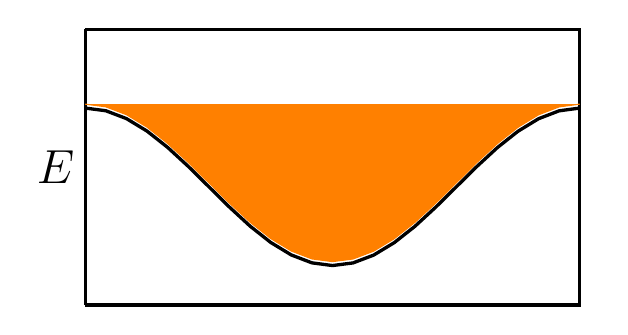
\begin{tikzpicture}[domain=0:6.28]
      \draw[very thick] (0, -2.5) -- (0,1) node[left, midway] {\LARGE $E$} ;
      \draw[very thick] (0, 1)-- (6.28,1) -- (6.28, -2.5) -- (0, -2.5);
      \draw[color=black, very thick] plot (\x,{-1+cos(\x r)}) node[right] {};
      \draw[color=orange, fill] plot (\x,{-0.95+cos(\x r)}) {};
  \end{tikzpicture}
  
            }
        \caption{Band Insulator}
        \end{figure}
    \end{column}
    \begin{column}[T]{.6\textwidth}
        \begin{figure}[h]
            \scalebox{1.4}{
            \input{diagrams/aklt_bare.tex}
            }
            \caption{Heisenberg AF Spin-1 chain}
        \end{figure}
    \end{column}
\end{columns}
\end{frame}
\newcommand{\kk}{\mathbf{k}}
\begin{frame}{Free Fermion Band Insulators}
\vskip-1.5cm
\begin{columns}[T]
\begin{column}[T]{0.65\textwidth}
\bi 
\item Crystaline, 0T insulators \\(including semiconductors)
%A good source of examples - column IV of periodic table, such as C, or in combination with column VI 
%(Columns I-III prefer to donate their valence electrons and form ionic bonds or metals)
%Microscopics are described well by
\item Tight-binding Hamiltonian 
$$
\mathcal{H}_{FF} =  \sum\limits_{<ij>}\sum\limits_{\alpha, \beta}-t_{\alpha, \beta} c^{\alpha \dagger}_{i} c_{j}^{\beta} - \mu \sum\limits_{i, \alpha} N_{i}^{\alpha} 
$$
%Diagonalize in momentum space to produce band picture, completely fill some lowest number of bands
\item Bloch Wavefunctions
$
\ket{u^{\alpha}_{\kk}}
$
%Low energy physics can be described by the Dirac Hamiltonian, with an effective mass for electron-like excitations, which looks in 2d like
\item Massive Dirac Hamiltonian 
$$
\mathcal{H}_{D}(\kk) = \kk_x \sigma_x + \kk_y \sigma_y + m_*\sigma_z
$$
%Describing a single conduction and valence band with a gap to pair production of quasi-electron+quasi-hole
\item Atomic-insulating like Wannier basis
%From Fourier transforming the Block wavefunctions
\ei 
\end{column}

\begin{column}[T]{0.35\textwidth}
\vskip3cm
\only<1>{
    \begin{figure}
        \includegraphics[width=\linewidth]{diagrams/GaNcrystal.jpg}
        \caption{Semiconductor GaN}
    \end{figure}
}    
\only<2>{
    \begin{figure}
        \includegraphics[width=\linewidth]{diagrams/GaNcrystal.jpg}
        \caption{Band Theory}
    \end{figure}
}
\only<3>{
    \begin{figure}
        \includegraphics[width=\linewidth]{diagrams/GaNcrystal.jpg}
        \caption{Dirac Band Theory}
    \end{figure}
}
\only<4>{
    \begin{figure}
        \includegraphics[width=\linewidth]{diagrams/GaNcrystal.jpg}
        \caption{Wannier Function}
    \end{figure}
}
\end{column}
\end{columns}
\end{frame}
\begin{frame}{Motivating Questions}
%from the classification of featureless insultors.
\vskip -1.5cm
\begin{block}{Existence}
Are there \textbf{constraints} on the existence of featureless insulators?
Can we \textbf{construct} featureless insulators when possible?
\\\vspace{1em}
{\em
Given a %particularly non-bravais 
lattice $\Lambda$, and an integer $m$, is there a featureless insulating phase of matter with $m$ particles per unit cell? 

%Our goal is to show exactly when you can construct a featureless state for every $m$ and $\Lambda$ - any additional constraints would be an extension of the LSM theorem.
}
%The Lieb-Schultz-Mattis theorem gives one such constraint - m must be an integer. But  
\end{block}
\begin{block}{Uniqueness}
How can we \textbf{distinguish} different classes of featureless insulators?
%Numerically, experimentally, etc.

Can we \textbf{enumerate} all such classes?\\
%Is there a general, mathematical principle for classifying featureless insulators?
\end{block}
\end{frame}
%\begin{frame}{Free Fermion Band Insulators}
\vskip-1.5cm
\begin{columns}[T]
\begin{column}[T]{0.65\textwidth}
\end{column}
\end{columns}
\end{frame}
%\note{Now lets talk about the physics of some common featureless phases}
\begin{frame}{Magnetization/Density Plateaus}
\vskip-1.5cm
Stable featureless insulators form magnetization or density plateaus

Example Hamiltonians and phase diagrams:
\only<1>{
\begin{block}{Band Insulators}
\vskip-0.5cm
$$
H_{FF} =  \sum\limits_{<ij>}-t_{ij} c^{\dagger}_i c_j - \mu \sum\limits_i N_i 
$$
\end{block}
\begin{columns}[T]
    \begin{column}[T]{.45\textwidth}
        \vskip-1cm
        \begin{figure}
        \centering
        \scalebox{0.7}{
         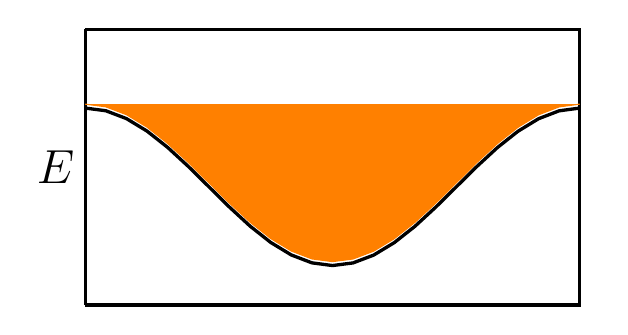
\begin{tikzpicture}[domain=0:6.28]
      \draw[very thick] (0, -2.5) -- (0,1) node[left, midway] {\LARGE $E$} ;
      \draw[very thick] (0, 1)-- (6.28,1) -- (6.28, -2.5) -- (0, -2.5);
      \draw[color=black, very thick] plot (\x,{-1+cos(\x r)}) node[right] {};
      \draw[color=orange, fill] plot (\x,{-0.95+cos(\x r)}) {};
  \end{tikzpicture}
  
        }
        \end{figure}
    \end{column}
    \begin{column}[T]{.55\textwidth}
    \vskip-0.7cm
    \bi 
    \item Symmetry protected band touchings can constrain existence of a band insulator
    \note{beyond integer filling LSM, on a given lattice tight-bonding model}
    \item Topological invariants can distinguish different types of band insulators
    \item Some invariants only make sense in the presence of additional symmetries ($\mathcal{T}, \mathcal{C}, \mathcal{I}$)
    \ei
    \end{column}
\end{columns}
}
\only<2>{
\begin{block}{Bose-Hubbard model}
\vskip-0.5cm
$$
H_{BH} = -J \sum\limits_{<ij>} b^{\dagger}_i b_j - \mu \sum\limits_i N_i + \frac12 V \sum\limits_i N_i (N_i-1)
$$
\end{block}
\begin{columns}[T]
    \begin{column}[T]{.45\textwidth}
        \vskip-1.2cm
        \begin{figure}
        \centering
        \includegraphics[width=4.5cm]{diagrams/bosehubbard2.png}
        \end{figure}
    \end{column}
    \begin{column}[T]{.55\textwidth}
    \vskip-0.7cm
    \bi 
    \item Interactions are always needed to stop Bose condensation
    \item Unlike free-fermions, not obvious how to construct fractional site filling insulators
    \item Tensor network states give us access to needed construction and to interacting invariants.
    \note{LSM inspired invariants}
    \ei
    \end{column}
\end{columns}
}

\only<3>{
\begin{block}{Haldane Phase for Spin-1 chains $(j=1, m=0)$}
\vskip-0.8cm
$$
H_{AKLT} = \sum\limits_{i} J \vec{S}_i\cdot \vec{S}_{i+1} + J' (\vec{S}_i\cdot \vec{S}_{i+1})^2 + D (S^z_i)^2+BS^x
$$
\end{block}
\begin{columns}[T]
    \begin{column}[T]{.45\textwidth}
        \vskip-1.2cm
        \begin{figure}
        \centering
        \includegraphics[width=\columnwidth]{diagrams/aklt2.png}
        \end{figure}
    \end{column}
    \begin{column}[T]{.55\textwidth}
    \vskip-0.8cm
    Two distinct featureless insulators:
    \bi 
    \item Large-D phase
    \bi 
    \item Contains product state wavefunction $\ket{\psi} = \ket{000...}$ 
    \ei
    \item Haldane phase
    \bi 
    \item Contains AKLT wavefunction $\ket{\psi} = \Sigma\ket{+00-0+...}$
    \ei 
        \begin{figure}[h]
            \hspace{-2cm}
            \scalebox{1.2}{
            \begin{frame}{MPS Example: AKLT State}
\vskip-1.5cm
\begin{block}{Haldane Phase for Spin-1 chains $(j=1, m=0)$}
\vskip-0.8cm
$$
H_{AKLT} = \sum\limits_{i} J \vec{S}_i\cdot \vec{S}_{i+1} + J' (\vec{S}_i\cdot \vec{S}_{i+1})^2 + D (S^z_i)^2+BS^x
$$
\end{block}
\begin{columns}[T]
    \begin{column}[T]{.45\textwidth}
        \vskip-1.2cm
        \begin{figure}
        \centering
        \includegraphics[width=\columnwidth]{diagrams/aklt2.png}
        \end{figure}
    \end{column}
    \begin{column}[T]{.55\textwidth}
    \vskip-0.8cm
    Two distinct featureless insulators:
    \bi 
    \item Large-D phase
    \bi 
    \item Contains product state wavefunction $\ket{\psi} = \ket{000...}$ 
    \ei
    \item Haldane phase
    \bi 
    \item Contains AKLT wavefunction $\ket{\psi} = \Sigma\ket{+00-0+...}$
    \ei 
        \begin{figure}[h]
            \hspace{-2cm}
            \scalebox{1.2}{
            \begin{frame}{MPS Example: AKLT State}
\vskip-1.5cm
\begin{block}{Haldane Phase for Spin-1 chains $(j=1, m=0)$}
\vskip-0.8cm
$$
H_{AKLT} = \sum\limits_{i} J \vec{S}_i\cdot \vec{S}_{i+1} + J' (\vec{S}_i\cdot \vec{S}_{i+1})^2 + D (S^z_i)^2+BS^x
$$
\end{block}
\begin{columns}[T]
    \begin{column}[T]{.45\textwidth}
        \vskip-1.2cm
        \begin{figure}
        \centering
        \includegraphics[width=\columnwidth]{diagrams/aklt2.png}
        \end{figure}
    \end{column}
    \begin{column}[T]{.55\textwidth}
    \vskip-0.8cm
    Two distinct featureless insulators:
    \bi 
    \item Large-D phase
    \bi 
    \item Contains product state wavefunction $\ket{\psi} = \ket{000...}$ 
    \ei
    \item Haldane phase
    \bi 
    \item Contains AKLT wavefunction $\ket{\psi} = \Sigma\ket{+00-0+...}$
    \ei 
        \begin{figure}[h]
            \hspace{-2cm}
            \scalebox{1.2}{
            \input{diagrams/aklt.tex}
            }
        \end{figure}

    \ei
    \end{column}
\end{columns}

\end{frame}
            }
        \end{figure}

    \ei
    \end{column}
\end{columns}

\end{frame}
            }
        \end{figure}

    \ei
    \end{column}
\end{columns}
}
% \only<3>{
% \bi
% \item Spin 3/2 Haldane Phase
% \ei
% $$
% H_{AKLT} = 
% $$
% \begin{figure}
% \centering
% \end{figure}
% }
\end{frame}
\subsection{Topological Band Insulators}
\begin{frame}{Frame Title}
\vskip-1.5cm

\end{frame}
\subsection{Bosonic Band Insulators?}
\begin{frame}{Frame Title}
\vskip-1.5cm

\end{frame}
\section{Featureless Boson Mott Insulators}
\begin{frame}{Frame Title}
\vskip-1.5cm

\end{frame}
\subsection{Honeycomb Featureless Insulator Proposal}
\newcommand{\hexa}{}
\begin{frame}[t]{Honeycomb Mott Insulators}
\framesubtitle{Proposed Wavefunction}
\vskip-1cm
Key insight\footnotemark: 'Center of charge' must lie at symmetric point

%For 1 boson/unit cell
%Similar idea called 'polarization' plays a part in the classifcation of Topological Crystalline Insulators
%Its a berry phase computed from band wavefunctions, determines a point in the unit cell
%If there is no such point in the lattice, its called non-symmorphic and you can't (proof rigorized in same way as LSM, flux threading) find a featureless insulator  
$$
\ket{\psi} = \prod\limits_{\varhexagon} \left(\sum\limits_{i \in \varhexagon} b^{\dagger}_i \right) \ket{\mathbf{0}}
$$
\only<1>{
\begin{figure}[h]
\scalebox{1}{
\input{diagrams/fbi1.tex}
}
\end{figure}
}

\only<2>{
\begin{figure}[h]
\scalebox{1}{
\input{diagrams/fbi2.tex}
}
\end{figure}
}

\only<3>{
\begin{figure}[h]
\scalebox{1}{
\input{diagrams/fbi3.tex}
}
\end{figure}
}

\only<4->{
\begin{figure}[h]
\scalebox{1}{
\documentclass[twocolumn,english,prb,showpacs]{revtex4-1}
\usepackage[colorlinks=true,urlcolor=blue,citecolor=blue,linkcolor=blue]{hyperref}
\usepackage[T1]{fontenc}
\usepackage[latin9]{inputenc}
\usepackage{amssymb}
\usepackage{graphicx}
\usepackage{amsmath,color}
\usepackage{mathrsfs}
\usepackage{float}
\usepackage{indentfirst}
\usepackage{babel}
\usepackage[sort&compress]{natbib}
\usepackage{color}

\newcommand{\bela}[1]{[\emph{\color{blue}{Bela: #1}}]}
\newcommand{\brayden}[1]{[\emph{\color{red}{Brayden: #1}}]}
\newcommand{\eqnref}[1]{Eq.~(\ref{#1})}

%\makeatletter

\begin{document}

\title{Not so featureless after all: symmetry protected order in an interacting boson state}

\author{Brayden Ware}

\author{Itamar}
\author{Sid}

\author{Bela Bauer}
\affiliation{Station Q, Microsoft Research, Santa Barbara, CA 93106-6105, USA}

\begin{abstract}
...
\end{abstract}
\maketitle

\section{Introduction}


\section{Conclusions}

\acknowledgements


\bibliography{fbi}


\end{document}

}
\end{figure}

%No valid Wannier functions, so we sacrifice 
Overlapping orbitals NOT orthogonal
%Or boson operators don't commute
}
\only<1-3>{\footnotetext[3]{\citep{Kimchi2012-lr}}}
\end{frame}
\begin{frame}{PEPS Construction of Honeycomb F.B.I.}
\vskip-1.5cm
A wavefunction written as a product of local operators acting on a product state can be turned into a tensor network.

\only<1>{
\begin{figure}[h]
\scalebox{1}{
% y=\sqrt{3/4}*(minimum size)/2
%

%http://tex.stackexchange.com/questions/6019/drawing-hexagons
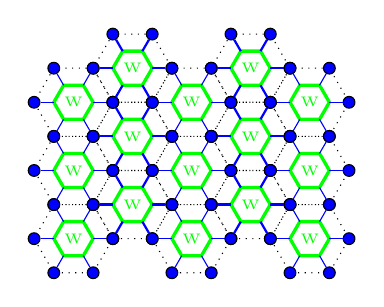
\begin{tikzpicture}[x=7.5mm,y=4.33mm]
  % some styles
  \tikzset{
    box/.style={
      regular polygon,
      regular polygon sides=6,
      minimum size=10mm,
      inner sep=0mm,
      outer sep=0mm,
      rotate=0,
     dotted,
     thin,
      black,
      draw
    }
  }
  \tikzset{
    bbox/.style={
      regular polygon,
      regular polygon sides=6,
      minimum size=7mm,
      %fill,
      inner sep=0mm,
      outer sep=0mm,
      rotate=0,
     % dotted,
     very thick,
     orange,
      draw
    }
  }
    \tikzset{
    wb/.style={
       regular polygon,
      regular polygon sides=6,
      minimum size=5mm,
      %fill,
      inner sep=0mm,
      outer sep=0mm,
      rotate=0,
     % dotted,
     very thick,
     green,
      draw
    }
  }
 \tikzset{boson/.style={circle=1pt,draw=black!100,fill=orange!100,inner sep=2pt}}
  \tikzset{dimer/.style={ellipse=1pt,draw=black!100,fill=orange!90,inner sep=2pt}}
    \tikzset{thindimer/.style={ellipse=1pt,draw=black!100,fill=orange!90,inner sep=1pt}}
\tikzset{peps/.style={circle=2pt,draw=black!100,fill=green!50,inner sep=3pt}}
\tikzset{bpeps/.style={circle=2pt,draw=black!100,thick,fill=green!50,inner sep=3pt}}
\tikzset{gamma/.style={circle=2pt,draw=black!100,fill=blue!50,inner sep=3pt}}
\tikzset{lambda/.style={rectangle,rotate=45,draw=black!100,fill=red!50,inner sep=2pt}}
\tikzset{operator/.style={circle=1pt,draw=black!100,fill=blue,inner sep=1.5pt}}

\foreach \i in {0,...,2} 
    \foreach \j in {0,...,2} {
    \pgfmathtruncatemacro{\x}{2*\i}
    \pgfmathtruncatemacro{\y}{2*\j}
            \node[box] (H\x\y) at (\x,\y) {};
             \node[wb] (W\x\y) at (\x,\y) {};
              \node[green] at (\x, \y) {\tiny W};
             \foreach \k in {1, ..., 6}{
             \node[operator] (D\x\y\k) at (H\x\y.corner \k) {};
             \draw[ blue] (W\x\y) -- (D\x\y\k);
             }
        }
\foreach \i in {0,1} 
    \foreach \j in {0,..., 2} {
        \pgfmathtruncatemacro{\x}{2*\i+1}
    \pgfmathtruncatemacro{\y}{2*\j+1}
   	  \node[box] (H\x\y) at (\x,\y) {};   
   	   \node[wb] (W\x\y) at (\x,\y) {};
   	    \node[green] at (\x, \y) {\tiny W};
             \foreach \k in {1, ..., 6}{
             \node[operator] (D\x\y\k) at (H\x\y.corner \k) {};
             \draw[thick, blue] (W\x\y) -- (D\x\y\k);
             }
        }


            %\foreach \k in {1,...,6}{
          %  \node[circle, label=above:\i, fill=red] at (H\i\j.corner \k) {};
           % }
%\node[circle, draw] at (H00.corner 1) {};
\end{tikzpicture}
}
\end{figure}

Virtual W-state on each plaquette used to synchronize the creation operators in the sum $\sum\limits_{i \in \varhexagon} b^{\dagger}_i$
$$\vket{W} = \vket{000001}+\vket{000010}+\vket{000100}+\vket{001000}+\vket{010000}+\vket{100000}$$

}

\only<2>{
\begin{columns}[T]
\begin{column}{0.5\textwidth}
\begin{figure}[h]
\scalebox{1.3}{
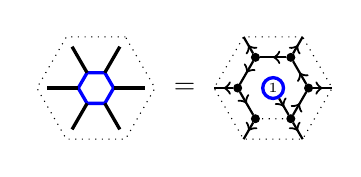
\begin{tikzpicture}[x=7.5mm,y=4.33mm]
\begin{scope}[decoration={
    markings,
    mark=at position 0.5 with {\arrow{>}}}
    ]
    
  \tikzset{
    box/.style={
      regular polygon,
      regular polygon sides=6,
      minimum size=15mm,
      inner sep=0mm,
      outer sep=0mm,
      rotate=0,
     dotted,
     thin,
      black,
      draw
    }
    }
      \tikzset{
    abox/.style={
      regular polygon,
      regular polygon sides=6,
      minimum size=9mm,
      inner sep=0mm,
      outer sep=0mm,
      rotate=0,
     dotted,
     thin,
      black,
      draw
    }
    }


    \tikzset{
    wb/.style={
       regular polygon,
      regular polygon sides=6,
      minimum size=4.5mm,
      %fill,
      inner sep=0mm,
      outer sep=0mm,
      rotate=0,
     % dotted,
     very thick,
     blue,
      draw
    }
  }
\tikzset{smalldot/.style={circle=1pt,draw=black!100,fill=black!100,inner sep=1pt}}
\tikzset{smallwdot/.style={circle=1pt, very thick, draw=blue!100,fill=white,inner sep=1pt}}

 \node[box] (H) at (0, 0) {};
\node[wb] (W) at (0,0) {};

\foreach \k in {1, ..., 6}{
             \node[inv] (D\k) at (H.corner \k) {};
             \draw[very thick, black] (W) -- (D\k);
             }
             
 \node[] at (1.5, 0){$=$};

 \node[box] (H3) at (3, 0) {};
 \node[abox] (H2) at (3, 0) {};
%\node[wb] (W) at (3,0) {\tiny W};
\foreach \k in {1, ..., 6}{
             \node[smalldot] (A\k) at (H2.corner \k) {};
             }

\foreach \k in {1,2,3,5}{
		\pgfmathtruncatemacro{\j}{\k+1}
            \draw[thick, postaction={decorate}] (A\k) -- (A\j);
             }
             \draw[thick, postaction={decorate}] (A6) -- (A1);
             
 \foreach \k in {1,2,3,4,5,6}{
            \draw[thick, postaction={decorate}] (A\k) -- (H3.corner \k);
             }
             
 \node[smallwdot](B) at (3, 0) {\tiny 1};
 \draw[thick, postaction={decorate}]  (B)--(A5);

\end{scope}
\end{tikzpicture}
}
\end{figure}
$$\vket{W} = \vket{100...}+...$$
\vskip-0.5cm
\bi 
\item W-State can be factored and put on hexagon sites
\item Each black directed string has either charge $0$ or $1$
\item Charge conserved
\ei 
\end{column}
\begin{column}{0.5\textwidth}
\begin{figure}[h]
\scalebox{1.5}{
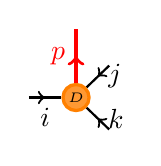
\begin{tikzpicture}[x=7.5mm,y=4.33mm]
\begin{scope}[decoration={
    markings,
    mark=at position 0.5 with {\arrow{>}}}
    ]
    

\tikzset{operator/.style={circle=1pt,draw=orange!100, very thick, fill=orange!80,inner sep=1pt}}
   
   \node[operator] (A) at (1, 0){\tiny $D$};
    \draw[thick, postaction={decorate}] (0.2, 0) --node[below]{$i$} (A);
    \draw[thick, postaction={decorate}] (5/3.2, 3/3.2) -- node[right]{$j$}(A);
    \draw[thick, postaction={decorate}] (5/3.2, -3/3.2) -- node[right]{$k$} (A);
    \draw[red, very thick, postaction={decorate}]  (A)-- node[left]{$p$}(1, 2);




\end{scope}
\end{tikzpicture}
}
\end{figure}
\vskip-0.3cm
\bi 
\item `Projects' the three virtual qubits coming into each vertex on to a state in physical Hilbert space
\item Physical state is either $\ket{0}, \ket{1}, \ket{2}, \ket{3}$
\item Charge conserved
\ei 
\end{column}
\end{columns}
}

\end{frame}
\section{Entanglement Spectra}
\subsection{CFT Identification}
\begin{frame}{Entanglement Spectra}
\vskip-1.5cm
\only<1>{
\begin{figure}
\includegraphics[width=\textwidth]{{interpolatedboson/new_plots/L_10_all_mom_10.pdf}}
\end{figure}
}
\only<2>{
\begin{figure}[hbctp]
\begin{center}
\includegraphics[width=\textwidth]{{interpolatedboson/new_plots/L_9_all_mom_10.pdf}}
\end{center}
\end{figure}}
\end{frame}
\begin{frame}{Finite Size Analysis of Spectra}
\vskip-1.5cm
\begin{columns}[T]
    \begin{column}{.4\textwidth}
        \bi 
        \item<1-> Topological entanglement entropy is 0 
        \item<2-> Low energy modes show gapless $1/L$ behavior
        \ei
    \end{column}
    \begin{column}{.6\textwidth}
    \vskip-.3cm
        \only<2>{
        \begin{figure}[hbctp]
        \centering
        \includegraphics[width=2.5in]{{interpolatedboson/a10/plots/EntanglementEnergyScaling2.pdf}}
        %\caption{Power law fits for the lowest three states above the ground state at momentum zero and lowest two states at momentum 1 in Figure \ref{fig:sc-EEFinitesize}. The $1/L$ scaling is a signature of a gapless (entanglement) Hamiltonian. The labeling of the states $\ket{e, m}$ or $j_{-1} \ket{e, m}$ is explained in the CFT section below.}
        %\label{fig:sc-EEScaling}
        \end{figure}
        }
    \end{column}
\end{columns}
\end{frame}
\include{slides/CFT_EE}
\begin{frame}{Conformal Tower}
\only<1>{
\begin{figure}
    \scalebox{1}{
        \input{diagrams/CFT_tower1.tex}
    }
\end{figure}
}
\only<2>{
\begin{figure}
    \scalebox{1}{
        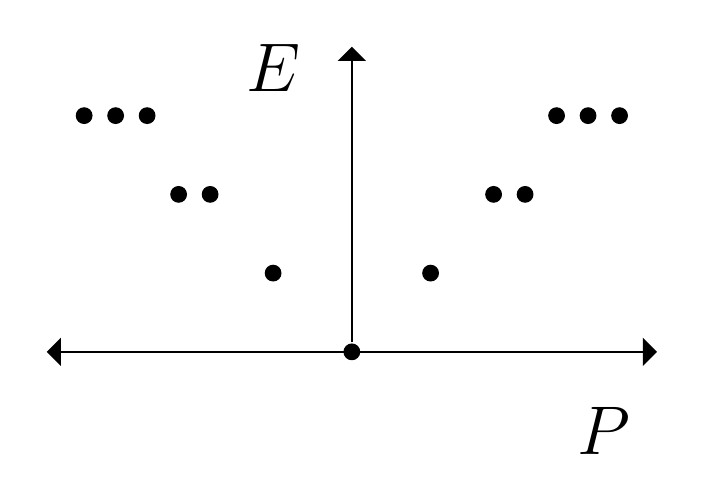
\begin{tikzpicture}
\tikzstyle{yaxis} = [-triangle 90]
\tikzstyle{xaxis} = [triangle 90-triangle 90]
\node[inv](A) at (-4, 0){};
\node[inv](B) at (4, 0){};
\draw[thick, xaxis] (A)-- (B);
\node at ($ (A) !.9! (B) +(0, -1)$) {\Huge $P$};
\node[inv](A) at (0, 0){};
\node[inv](B) at (0, 4){};
\draw[thick, yaxis] (A)--(B);
\node at ($ (A) !.9! (B) +(-1, 0)$) {\Huge $E$};

\tikzset{spec/.style={circle=2pt,draw=black!100,fill=black!100,inner sep=2pt}}
\node[spec] at (0, 0){};
\node[spec] at (1, 1){};
\node[spec] at (1.8, 2){};
\node[spec] at (2.2, 2){};

\node[spec] at (2.6, 3){};
\node[spec] at (3.0, 3){};
\node[spec] at (3.4, 3){};

\node[spec] at (-1, 1){};
\node[spec] at (-1.8, 2){};
\node[spec] at (-2.2, 2){};

\node[spec] at (-2.6, 3){};
\node[spec] at (-3.0, 3){};
\node[spec] at (-3.4, 3){};


%\node[spec] at (-1, 1){};
%\node[spec] at (0, 2){};

%\node[] at (3, -1.5){\LARGE Band metal};
%\node[] at (3, 1.5){\LARGE Band insulator};
%\draw[] (0.5, 0) -- (5.5, 0);
\end{tikzpicture}
    }
\end{figure}
}
\only<3>{
\begin{figure}
    \scalebox{1}{
        \input{diagrams/CFT_tower3.tex}
    }
\end{figure}
}
\only<4>{
\begin{figure}
    \scalebox{1}{
        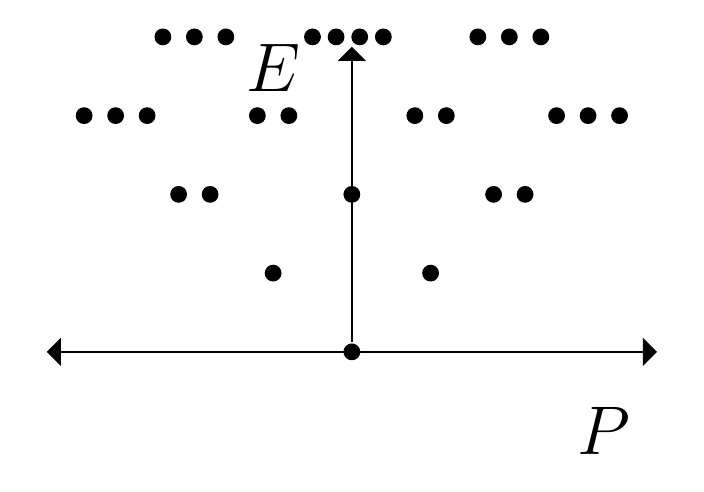
\begin{tikzpicture}
\tikzstyle{yaxis} = [-triangle 90]
\tikzstyle{xaxis} = [triangle 90-triangle 90]
\node[inv](A) at (-4, 0){};
\node[inv](B) at (4, 0){};
\draw[thick, xaxis] (A)-- (B);
\node at ($ (A) !.9! (B) +(0, -1)$) {\Huge $P$};
\node[inv](A) at (0, 0){};
\node[inv](B) at (0, 4){};
\draw[thick, yaxis] (A)--(B);
\node at ($ (A) !.9! (B) +(-1, 0)$) {\Huge $E$};

\tikzset{spec/.style={circle=2pt,draw=black!100,fill=black!100,inner sep=2pt}}
\node[spec] at (0, 0){};
\node[spec] at (1, 1){};
\node[spec] at (1.8, 2){};
\node[spec] at (2.2, 2){};

\node[spec] at (2.6, 3){};
\node[spec] at (3.0, 3){};
\node[spec] at (3.4, 3){};

\node[spec] at (0-1, 0+1){};
\node[spec] at (1-1, 1+1){};
\node[spec] at (1.8-1, 2+1){};
\node[spec] at (2.2-1, 2+1){};

\node[spec] at (2.6-1, 3+1){};
\node[spec] at (3.0-1, 3+1){};
\node[spec] at (3.4-1, 3+1){};

\node[spec] at (0-2.2, 0+2){};
\node[spec] at (1-2.2, 1+2){};
\node[spec] at (1.8-2.3, 2+2){};
\node[spec] at (2.2-2.1, 2+2){};

\node[spec] at (0-1.8, 0+2){};
\node[spec] at (1-1.8, 1+2){};
\node[spec] at (1.8-2, 2+2){};
\node[spec] at (2.2-1.8, 2+2){};

\node[spec] at (-2.6, 3){};
\node[spec] at (-3.0, 3){};
\node[spec] at (-3.4, 3){};

\node[spec] at (-2.6+1, 4){};
\node[spec] at (-3.0+1, 4){};
\node[spec] at (-3.4+1, 4){};


\end{tikzpicture}
    }
\end{figure}
}
\end{frame}
\begin{frame}{Level identification in CFT spectra}
\vskip-1.5cm
\only<1>{

To make a precise comparison with the free-boson CFT, we'll need to solve for (or look up) the solution of this model.

The free-boson CFT is created from the Lagrangian 
$$ \mathfrak{L} = \frac{g}{2}\int dt \int\limits_0^L dx ( \frac{1}{v^2}(\partial_t \phi)^2 - (\partial_x \phi)^2)$$
and with the compatified field identification
$$ \phi \equiv \phi + 2\pi R$$
and placed on the circle of circumference $L$ with periodic boundary conditions
$$ \phi(x) \equiv \phi(x+L).$$
}

Canonically quantize!
\end{frame}
\begin{frame}{Level identification in CFT spectra}
\vskip-1.5cm
\begin{figure}
\scalebox{0.5}{
\input{diagrams/CFT_schematic3.tex}
}
\end{figure}
\end{frame}
%\newcommand{\uL}{\mathbf{L_0}}
%\newcommand{\bL}{\mathbf{\bar{L}_0}}
\begin{frame}{Level identification in CFT spectra}
\vskip-1.5cm

\end{frame}
\begin{frame}{Open questions and speculation}
\bi
\item Parent Hamiltonian - Construct or obstruction?
\item Symmetry group/groups that protect edge?
\item Correspondence between bulk perturbations and edge perturbations?
\item Nearby phase transitions? 
\item Is the edge `anomalous'? 
\item We can put lots of known SPTs in tensor networks. What should we do next?
\item Can we represent transfer matrix as a MPO for efficient contraction?
\item Tensor Network RG?
\ei 

\end{frame}
\section*{}

\begin{frame}
  \frametitle{Resources}
  %\framesubtitle{If you want to improve this style}
  \begin{thebibliography}{10}

  \beamertemplatearticlebibitems

  \bibitem{PEPS}
  A Practical Introduction to Tensor Networks
    \newblock {\tt Orus, R. A Practical Introduction to Tensor Networks: Matrix Product States and Projected Entangled Pair States. arXiv [cond-mat.str-el] (2013). at <http://arxiv.org/abs/1306.2164> 
}

  \end{thebibliography}
\end{frame}

\frame{
  \vspace{2cm}
  {\huge Questions ?}

  \vspace{3cm}
  \begin{flushright}
    Brayden Ware

    \structure{\footnotesize{brayden@physics.ucsb.edu}}
  \end{flushright}
}

\frame{
  \vfill
  \centering
  \highlighton{
  \usebeamerfont*{frametitle}Bonus slides

  \usebeamerfont*{framesubtitle}Bonus slides
  }
  \vfill
}


\end{document}
